\subsection{Industrial vibration monitoring solutions}
Two of the most established innovators in the field od real-time machine monitoring are Bently Nevada and Emerson, which offer a wide range of wireless and hardwired solutions along with corresponding data visualization. Their customers come from large-scale industries sectors such as power generation, mining and steel production. However the visualization provided typically remains limited to raw amplitude plots, which require high domain expertise and do not offer a an intuitive overview of machine health. 
\begin{figure}[H]
\centering
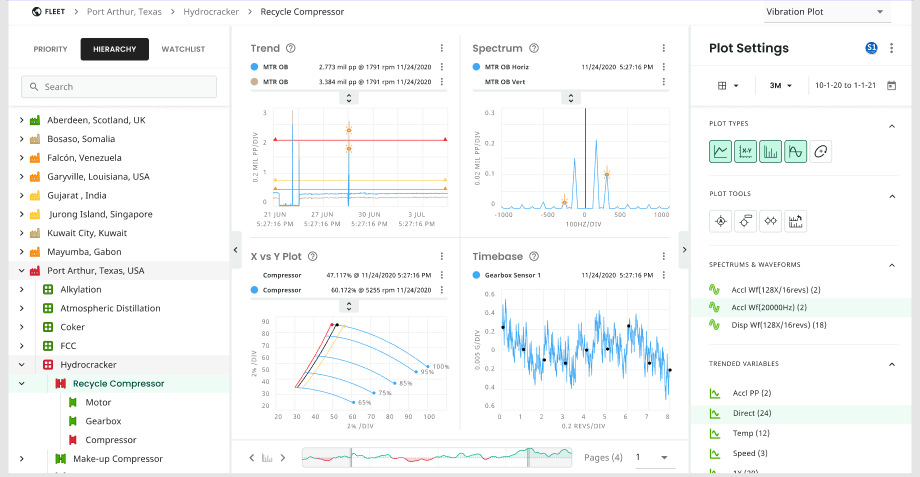
\includegraphics[width=0.8\textwidth]{figures/test2.png}
\caption{Dashboard example from a commercial condition-monitoring platform.\parencite{snyder2021roadmap}}
\label{fig:dashboardBentlyNevada}
\end{figure}
It must be pointed out that the data shown in figure \ref{fig:dashboardBentlyNevada} does not represent sensible customer data but rather only plots mock data for demonstration purposes provided by the vendor.
The dashboard provides an example offered by such platforms: \textcite{snyder2021roadmap} a full complement of diagnostic plots is provided, including polar, orbit, waveform, spectrum, waterfall, air gap, X-Y, multivariable trend, bode and amplitude phase time, and others. While this offers comprehensive coverage, no plot is designed ti make periodic behavior immediately visible at first sight. In contrast the system requires to interpret a specific aspect of the signal separately. A fingerprint plot such as the ones produced by principal component analysis would be a valuable extension to the already established workflows offering a better overview of periodicity and structural changes that normally would require cross referencing across multiple specialized plots.